\documentclass[tikz,border=10pt]{standalone}
% Scale s = 0.015066 cm/px, origin at ink-bbox centre (302.5, 222.5)
\begin{document}
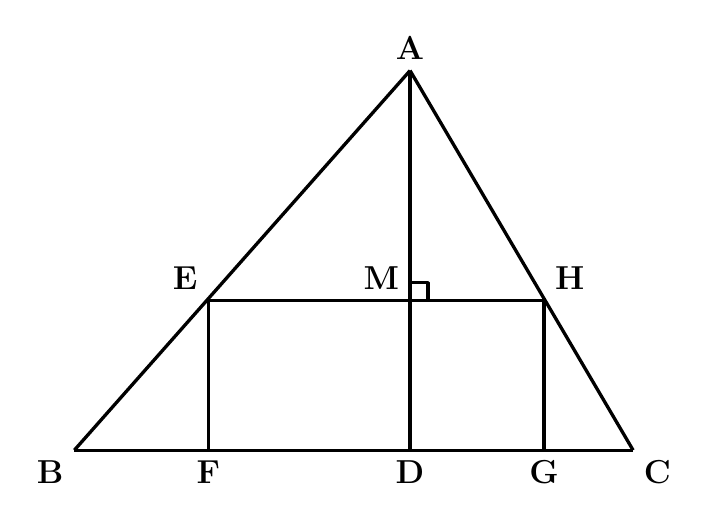
\begin{tikzpicture}[line width=1.2pt, line join=round, font=\fontsize{12}{14.4}\selectfont]
  % Named coordinates (converted from pixels)
  \coordinate (A) at (0.7156,2.4482);
  \coordinate (B) at (-3.5481,-2.3729);
  \coordinate (C) at (3.5481,-2.3729);
  \coordinate (D) at (0.7156,-2.3729);
  \coordinate (E) at (-1.8456,-0.4746);
  \coordinate (F) at (-1.8456,-2.3729);
  \coordinate (G) at (2.4181,-2.3729);
  \coordinate (H) at (2.4181,-0.4746);
  \coordinate (M) at (0.7156,-0.4746);

  % Solid black segments (geometry unchanged)
  \draw (A) -- (B);
  \draw (B) -- (C);
  \draw (C) -- (A);
  \draw (A) -- (D);
  \draw (E) -- (H);
  \draw (E) -- (F);
  \draw (H) -- (G);

  % Right-angle mark at M (between MA up and MH right)
  \draw (M)++(0,0.229) -- ++(0.229,0) -- ++(0,-0.229);

  % Labels: upright bold serif, correct bindings (C at bottom-right, H at (463,254), A only at apex)
  \node[above] at (A) {\textbf{A}};
  \node[below left] at (B) {\textbf{B}};
  \node[below right] at (C) {\textbf{C}};
  \node[below] at (D) {\textbf{D}};
  \node[above left] at (E) {\textbf{E}};
  \node[below] at (F) {\textbf{F}};
  \node[below] at (G) {\textbf{G}};
  \node[above right] at (H) {\textbf{H}};
  \node[above left] at (M) {\textbf{M}};
\end{tikzpicture}
\end{document}